\documentclass[letterpaper,12pt,fleqn]{article}
\usepackage{matharticle}
\pagestyle{empty}

\begin{document}

\section*{The Real Numbers}

\subsection*{Counting}

\begin{itemize}[left=0in]
\item The archaeological record contains sticks/bones with marks on them, indicating that prehistoric man was
  counting.
  \begin{center}
    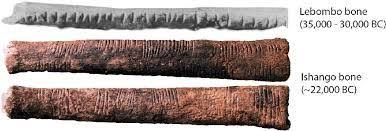
\includegraphics{bones}
  \end{center}

\item When counting, an object in the real world is associated with a mark on the stick/bone.
  \begin{center}
    \begin{tikzpicture}
      \node (S) at (2,4) {
\includegraphics[scale=0.5]{sheep}};
      \draw (0,0) rectangle (8,1);
      \foreach \i in {0.25,0.5,...,2.0}{
        \draw [red] (\i,0.25) -- (\i,0.75);
      }
      \draw [dashed,->] (S) to (0.75,0.75);
    \end{tikzpicture}
  \end{center}
  
\end{itemize}

\subsection*{The Natural Numbers}

\subsection*{The Integers}

\subsection*{The Rational Numbers}

\subsection*{The Irrational Numbers}

\subsection*{The Real Numbers}

\end{document}
